In the United States, and across the free world, politics has always been
adversarial. Among English speakers, we often metaphorically structure 
our politics as physical conflict. In this work we show that there are detectable
transitions where political events increase the use of figurative violence
in such political discourse. Part of this work is specifically interested in
mapping the subtleties of the use of metaphorical violence in the tradition of
conceptual metaphor theory initiated by the seminal work by \citeA{Lakoff1980}.
A more fundamental theoretical and methodological contribution is made here
in the course of analyzing United States' political discourse as a 
complex dynamical system as broadly suggested by \citeA{Cameron2006}.

Our cognitive corpus linguistics approach allows us to study metaphor 
\textit{in the wild}, as opposed to studying literary metaphor. Much of 
our everyday speech is figurative. The metaphors, and other figurative 
devices, we use can generally be traced to embodied experiences. There is a
growing wealth of evidence that our minds access and simulate such 
embodied experiences when comprehending metaphorical statements 
\cite{Gibbs2008}. 

Conventional conceptual metaphors like \textsc{kindness is warmth} are instantiated
in utterances such as ``I don't know what I did to make him act so
cold towards me,'' or ``she's a very warm person, a joy to be around.'' 
These are so fundamental to our understanding of social situations that
an utterance need not be made, but such conceptual metaphors still structure
our inner thoughts.
To take just one of many examples, a psycholological 
experiment asked one group of participants to think of a time when they were
accepted into a social group, while the other group of participants were asked
to think of a time when they were blocked out of a social group. 
All participants were then asked to estimate the controlled 
temperature in the room.  Participants who thought of social acceptance
gave significantly higher estimates of room temperature than the other group
\cite{Lakoff2014, Zhong2008}.

To summarize, metaphor is important to understanding cognition because 
\begin{enumerate}
    \item Metaphor (conceptual or uttered) bridges abstract ideas and physical experience \cite{Jamrozik2015}
  \item The use and comprehension of metaphor recruits language brain regions not normally 
    involved in language use and comprehension
  \item By studying how people use metaphor, we can understand how concepts
    are related and organized in their mind
\end{enumerate}
At this point, we can better understand why studying the nature of metaphors
that arise in politics would be important. Specifically, in the case of
metaphorical violence, we gain insight into the bitter, embattled feelings
that accompany elections in the United States. If \textsc{politics is war},
or more generally \textsc{politics is a fight}, then we deduce that our
fight-or-flight response would be recruited for comprehension of utterances
of violent framings of political debate and decision-making, such as voting.
Such claims are supported by results demonstrating there is a relationship
between aggressiveness, support for state violence or violence against authority, 
violence metaphors in political speeches, and voter turnout \cite{Kalmoe2012}.
Furthermore, \citeA{Westen} reviews many instances where political
participation decisions are made not through deliberative reasoning, but by
split-second, unconscious, refelxive reactions.
By first understanding the dynamics of such language use and their underlying
cognitive mechanisms, we can work towards
alternatives that do not require the recruitment of our most primitive 
cognitive circuitry. 
For example, adapting an example from \citeA[p. 139]{Lakoff1980}, we might
advocate for utterances that emerge from the conceptual metaphor
\textsc{politics is a collaborative work of art}. As we show in this paper,
the timing of such efforts could be of utmost importance.


\subsection{Data of the ``complex dynamical system''}

We analyzed a corpus built from scraping the Internet Archive's 
\href{http://archive.org/tv/details}{TV News Archive} for closed captioning.
While we could possibly have scraped transcripts directly from cable news
websites, the Internet Archive also provides a wealth of metadata along with
closed captioning all from one source, simplifying the process. Also transcripts
may have been edited, while the Internet Archive's resources were recorded
at the time of airing. This corpus represents the raw observations of what we
take as our complex dynamical system: English-language cable news productions
from the United States. This system is but a manifold of a larger, 
more complex system,
the population of the United States making the choice of who to vote for. 
Cable news serves as
a nicely-situated proxy in that it simultaneously provides and creates
a common ground between politicians/political campaigns and the voting public.
On the one hand, cable news producers must first 
interpret events in an way meaningful and interesting to themselves \cite{Clark1996}. 
Then, cable news producers must transmit that information to viewers in a
way that satisfies a show's sponsors and resonates
with the viewers. As discussed above, metaphor often provides
a ready-made conduit that increases the rate of information consumption by
viewers. For this reason, metaphorical violence describing the 2016 election
process is ubiquitious across the three networks studied: MSNBC, Fox News, and
CNN. But, the exact nature of which violent words or phrases are used changes
for each network, and ostensibly for each program on the network. Novel 
software, explained further in Section \ref{sec:Methods}, 
was used to search the corpus for violent words and phrases, which may have been
used figuratively or not, and possibly related to the election or not.
These results were then input to a web interface, also newly developed in 
conjunction with this project, where analysists determined whether or not the
usage was figurative and related to the election, along with other important
scientific data, explained further in Section \ref{sec:Methods}. 
From this coding, we counted the number of times figurative violence was 
used in each program airing, for each violet word or phrase, termed 
\textit{facet}, for each day. As an example of the data we collected, the 
total number of figurative usages across shows of \textit{attack}, \textit{hit}, and
\textit{beat}, the three most common, are shown in Figure \ref{fig:timeseries}. 
To better situate these counts, the three debates and the election are drawn
as dashed vertical lines. In addition to daily counts we also show the 7-day
moving average of usage. This gives us better intuition of the overall trend
of usage.

\begin{figure*}
\begin{center}
  % \vspace*{-.55in}
  \hspace*{-.25in}
  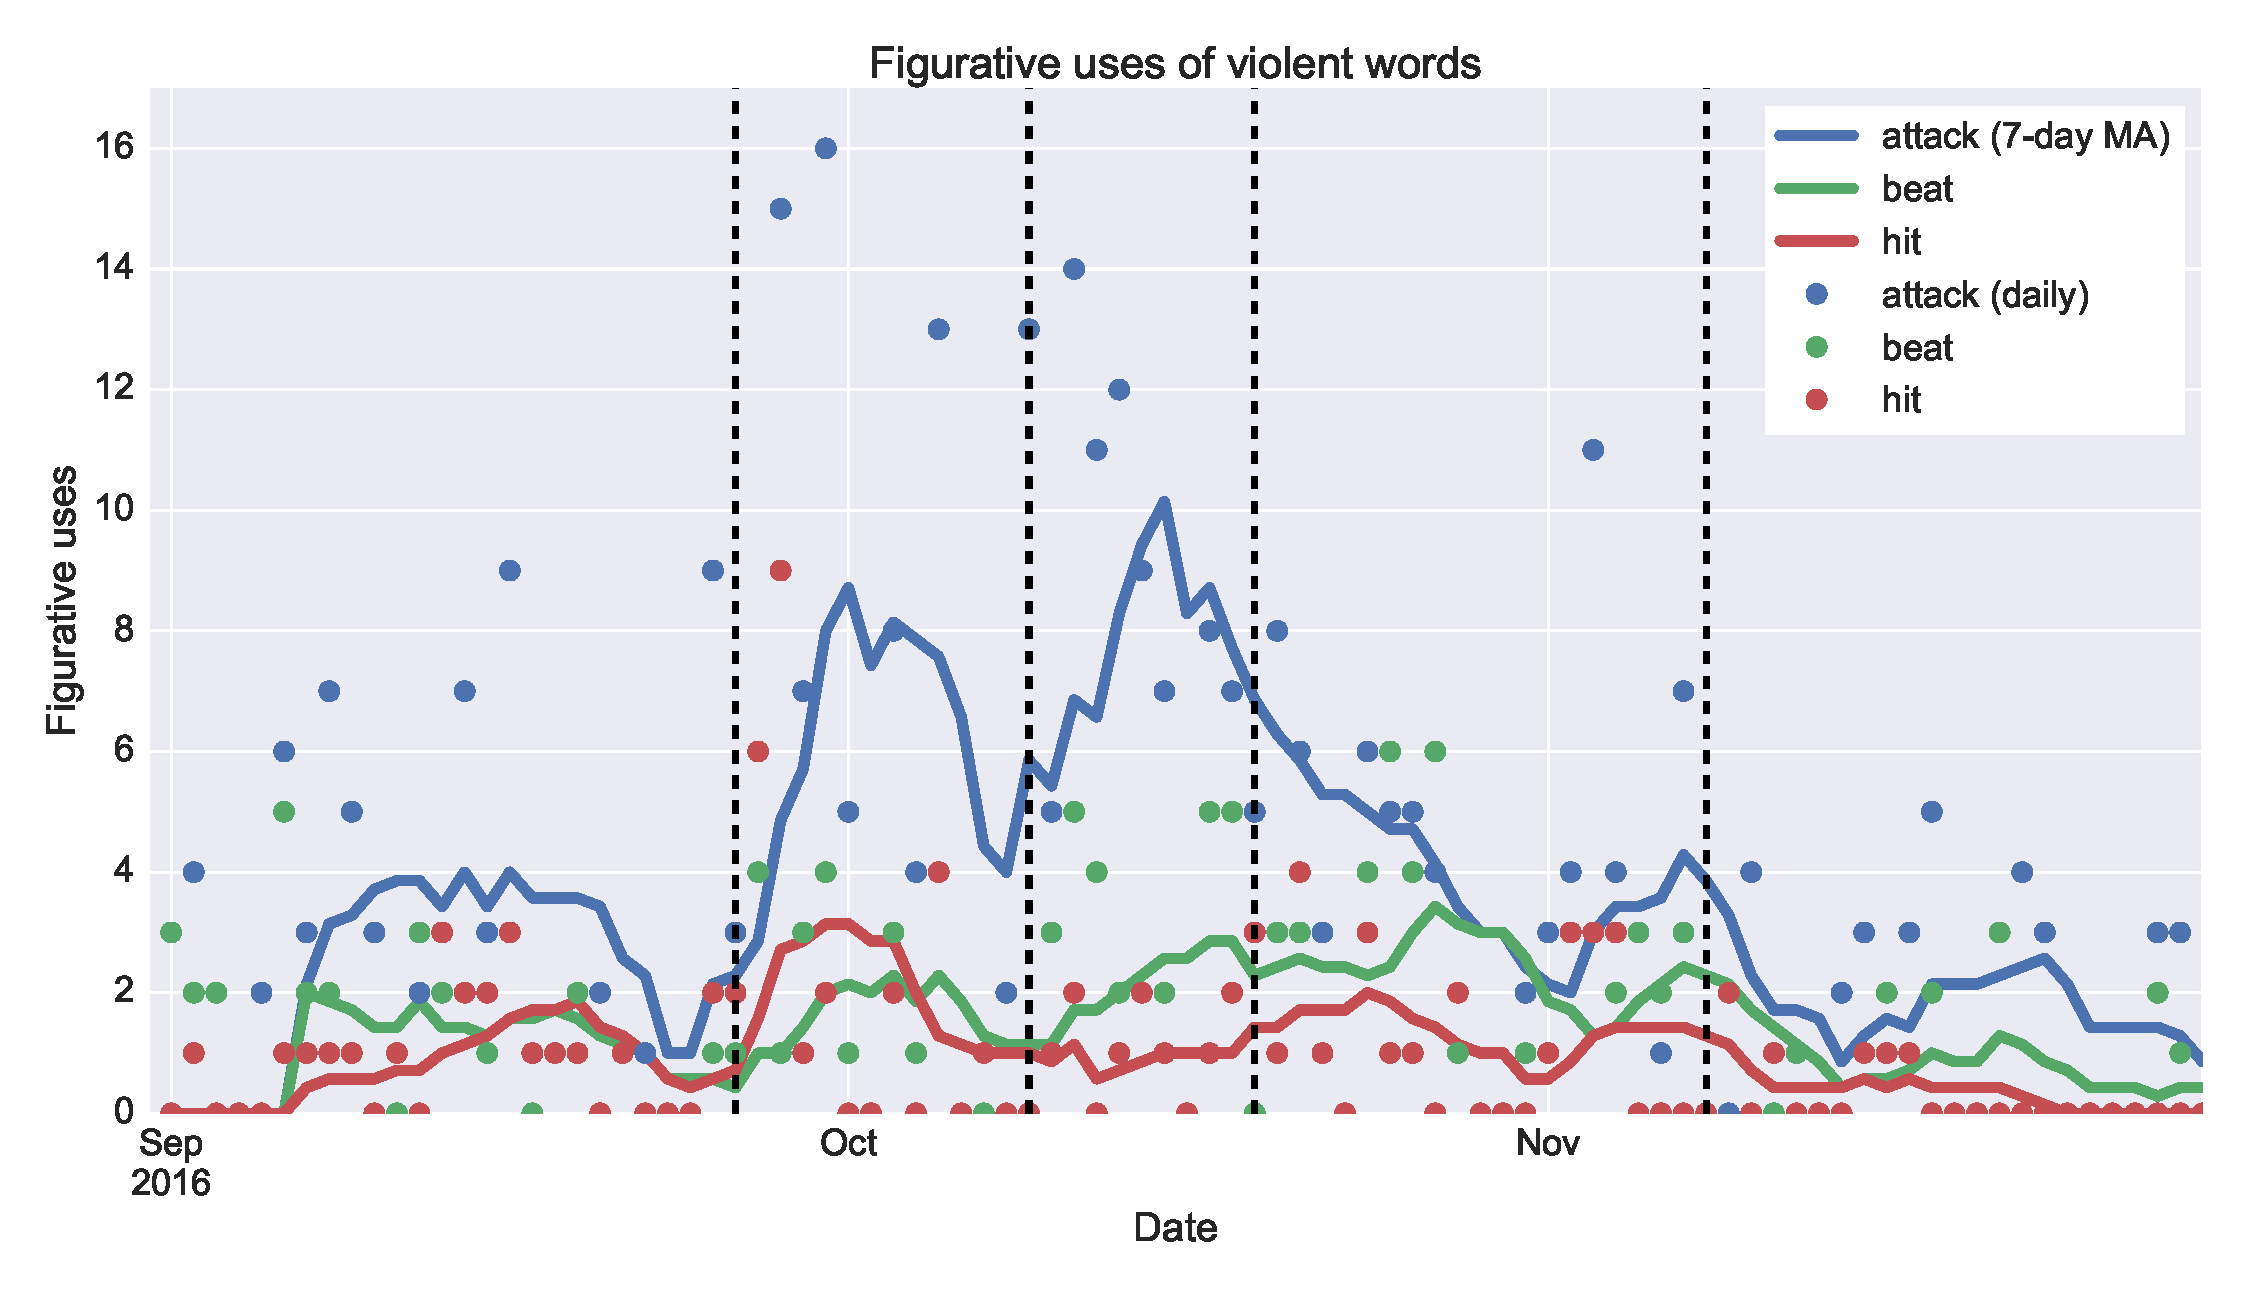
\includegraphics[width=\textwidth]{figures/fig_uses_violent_words-FIG1.pdf}
\end{center}
\caption{
  7-day moving average and daily counts of the figurative uses of the three-most
  used violent words in figurative constructions. Uses come from a variety of
  conceptual metaphors which more or less reduce to 
  \textsc{politics is a physical fight}. The first three dashed 
  vertical lines are the dates of the presidential debates, 
  September 26, October 9, and October 19, 2016. The last dashed
  line is election day, November 8, 2016.
}
\label{fig:timeseries}
\end{figure*}

\subsection{Theoretical and Methodological Contribution}
\label{sub:Theoretical-and-Methodological-Contribution}

Following the bold, but somewhat underdeveloped, proposal of \citeA{Cameron2006},
we consider the corpus as emergent behavior from a complex dynamical system \cite{Beer2000}.
There has been accelerating interest in connecting behavioral language data,
including corpora-from-the-wild. For example, \citeA{Gibbs2012a} explores 
the coupling between agents and their environments. 
In this work, Gibbs and Van Orden argue that pragmatic choice is an
emergent property of a system operating in a state of self-organized 
criticality. Language evolution is being studied from a dynamical systems perspective, 
where tendencies for change
can be understood to emerge from inconsistencies or inefficiencies in a 
language, or from outside influence \cite{Dale2016}. Also, there has been decades of interest
in the dynamical systems related to motor skills \cite{Haken1985}, speech 
production \cite{Kelso1986}, neural dynamics \cite{Chialvo2010}, and more
\cite{Spivey2007}. 

The contribution of this paper is that we use the complex dynamical systems
framing in order to answer an important question: can we meausre the
impact of cultural
events, specifically the presidential debates and the election, on the
frequency of usage of figurative violence on cable news? As discussed before,
cable news represents a proxy for the cognition of large segments of the
population. Thus we can gain insight to collective cognitive dynamics among
the English-speaking voting population of the United States. Specifically,
assuming there is an effect of these cultural events on figurative violence usage,
we want to know when the phase transitions occur and on what timescale do they
occur? There seem to be three equally valid \textit{a priori} hypotheses for
the timing of phase transitions. First, one might expect usage of figurative
violence to precede the onset of debates and the election in expectation of the
metaphorical ``war'' and ``fights'' to follow. Or, the increase in usage
might lag behind the beginning of debates, and emerge in response to a 
critical level of political argumentation, debate, etc., has been reached.
A third, less probable, hypothesis could be that the phase transition occurrs
exactly on the same date as one of the four cultural events we identified.
Borrowing further from dynamical systems theory, we show that the phase
transitions can have a degree of transience. This manifests itself in multiple
dates having close probabilities of resulting in the best model for segmenting
the data into phases.

\subsection{Outline}
\label{sub:Outline}

The rest of the paper is organized as follows. In Section \ref{sec:Methods}
the corpus-building, metaphor-coding, and analysis software is presented,
along with the statistical methods used for locating the phase transitions.
In Section \ref{sec:Results} we show that there are two strong candidates
for phase transitions in frequency of figurative violence usage, but one of
them shows more transience than the other. Finally, we discuss both the
theoretical and practical importance of our findings in the context of
increasing animosity and polarization in United States politics.

